\documentclass[10pt]{amsart}
%\include{amsmath}
\usepackage{mathtools}
\usepackage{amsmath}  
\usepackage{amssymb}  % gives you \mathbb{} font
\usepackage{dsfont}	% gives you \mathds{} font

%                   Math Blackboard Bold Symbols

\newcommand\Cb{\mathds{C}}
\newcommand\Eb{\mathds{E}}
\newcommand\Fb{\mathds{F}}
\newcommand\Gb{\mathds{G}}
\newcommand\Ib{\mathds{I}}
\newcommand\Pb{\mathds{P}}
\newcommand\Qb{\mathds{Q}}
\newcommand\Rb{\mathds{R}}
%\newcommand\Zb{\mathds{Z}}
\newcommand\Nb{\mathds{N}}
\newcommand\Vb{\mathds{V}}
\newcommand\Ub{\mathds{U}}

\usepackage[shortlabels]{enumitem}
\usepackage{amssymb}
\usepackage{bbm}
\usepackage{cancel}
\usepackage{graphicx,subfig}

\graphicspath{ {./images/} }

\newcommand{\D}{\mathrm{d}}
\DeclareMathOperator{\E}{e}
\DeclareMathOperator{\I}{i}


\begin{document}

\noindent
\text{Hunter Lybbert} \\
\text{Student ID: 2426454} \\
\text{11-22-24} \\
\text{AMATH 561}
\title{Problem Set 7}
\maketitle

{\it Note: Exercises 1-4 are from Matt Lorig's
notes (link on course website).}
\\

\noindent {\bf 1.} Exercise 4.1. \\
A six-sided die is rolled repeatedly. Which of the following are Markov chains? For those
that are, find the one-step transition matrix.\\

\begin{enumerate}[(a)]
\item $X_n$ is the largest number rolled up to the $n$th roll. \\

\noindent
\textit{Solution:} \\
It helps me to visualize this graphically. 
Let each state be a node with directed edges going from a given state to all reachable states from the current state.
\begin{figure}[h]
	\centering
	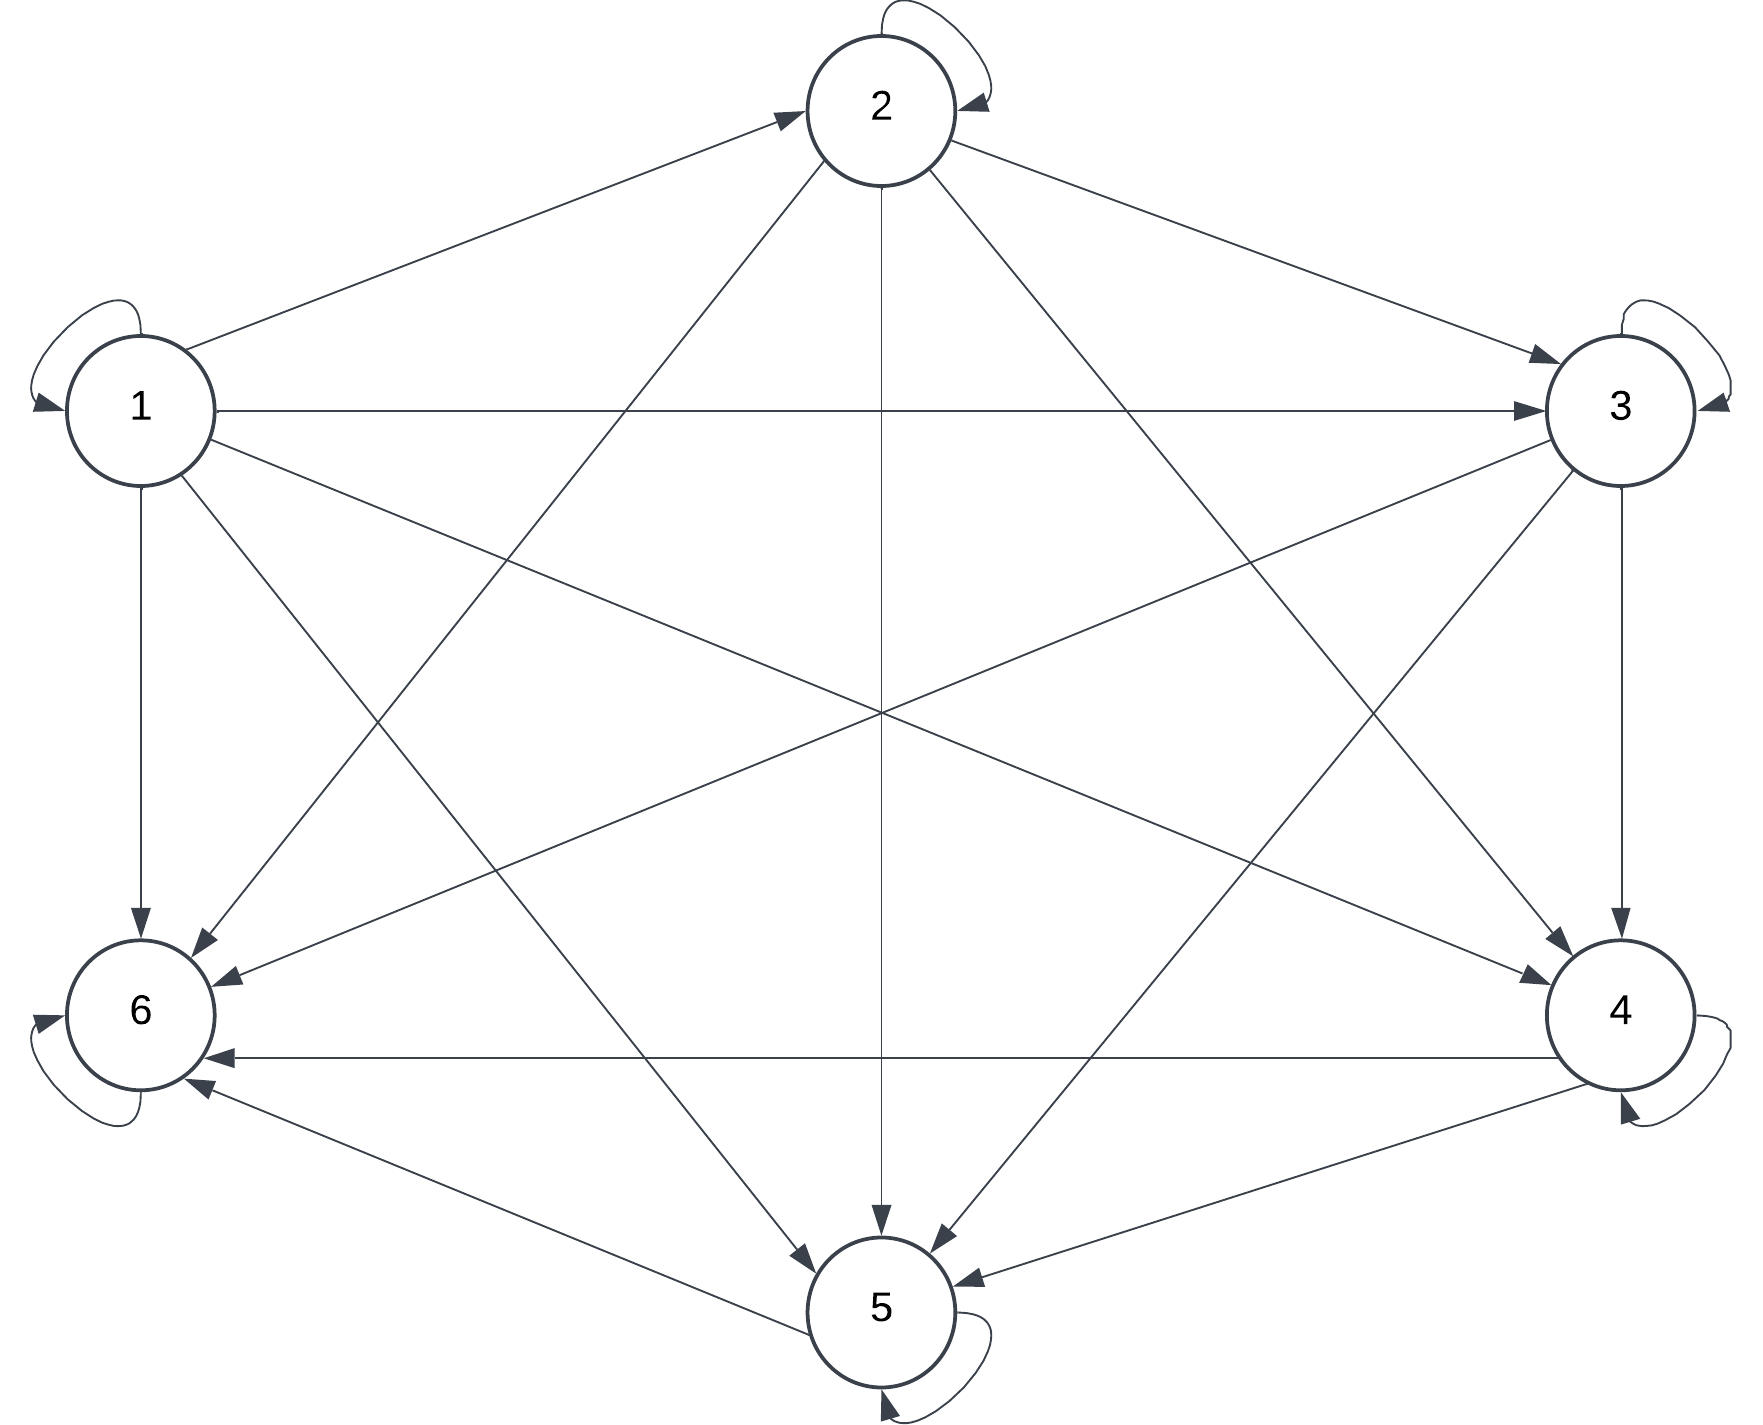
\includegraphics[scale=0.5]{one_part_a_markov_graph.png}
	\caption{
		A graphical representation of the Markov Chain in problem 1 part (a).
	}\label{fig:f1}
\end{figure}
If each directed edge in Figure \ref{fig:f1} is equally likely, then we can construct the following transition matrix
\begin{align*}
P = 
\begin{bmatrix}
1 /6 & 1 /6 & 1 /6 & 1 /6 & 1/6 & 1/6 \\
0 & 1/5 & 1/5 & 1/5 & 1/5 & 1 /5 \\
0 & 0 & 1/4 & 1/4 & 1/4 & 1/4 \\
0 & 0 & 0 & 1/3 & 1/3 & 1/3 \\
0 & 0 & 0 & 0 & 1/2 & 1/2 \\
0 & 0 & 0 & 0 & 0 & 1 \\
\end{bmatrix}.
\end{align*}
From the transition matrix it is easy to see this is a Markov chain.
This is due to the fact that the rows sum to $1$ and the probability of moving to a new state only depends on our current state. \\
\qed \\


\item $X_n$ is the number of sixes rolled in the first $n$ rolls. \\

\noindent
\textit{Solution:} \\
The transition matrix for this scenario can be written as
\begin{align*}
P =
\begin{bmatrix}
5/6 & 1/6 & 0 & 0 & \dots \\
0 & 5/6 & 1/6 & 0 & \dots \\
0 & 0 & 5/6 & 1/6 & \ddots\\
\vdots & \vdots & \ddots & \ddots & \ddots\\
\end{bmatrix}.
\end{align*}
Since we can write $X_n = X_{n - 1} + \xi_n$ where $\xi_n$ is 1 if the $n$th role is a 6 or 0 otherwise.
Therefore $\xi_n$ is Bernoulli distributed with probability of success $p = 1/6$.
Let the current state be denoted as $\ell$.
The state space is $\mathbb N \cup \{0\}$.
Furthermore we can say if $X_n = \ell$ we denote the following
$$
P(X_{n + 1} = \ell + 1 | X_n = \ell) = 1 / 6
$$
if the next role is a 6 and
$$
P(X_{n + 1} = \ell | X_n = \ell) = 5 / 6
$$
if the next role is not a 6.
Graphically that can be represented as seen in Figure \ref{fig:f2}
\begin{figure}[h]
	\centering
	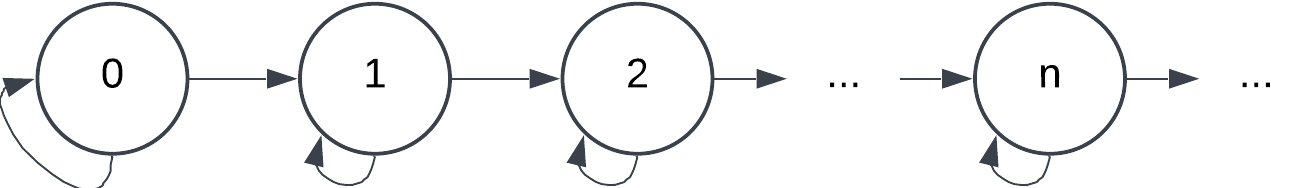
\includegraphics[scale=0.5]{one_part_b_markov_graph.png}
	\caption{
		A graphical representation of the Markov Chain in problem 1 part (b).
	}\label{fig:f2}
\end{figure}
Where the self returning edge has probability $5/6$ and the edge advancing from one state to the next higher state has probability $1/6$.
Now we can conclude this is a Markov chain because the probability of moving to a particular state is only determined by the current state we are in.
Additionally the rows of our matrix sum to 1 which satisfies our other criteria. \\
\qed \\


\item At time $n$, $X_n$ is the time since the last six was rolled. \\

\noindent
\textit{Solution:} \\
Each step is $5/6$ chance of not rolling a 6 therefore increasing $X_n$ and a $1/6$ chance of rolling a 6 therefore returning to the beginning state.
If I may say so myself, this is depicted clearly in the directed graph in Figure \ref{fig:f3}. \\
\begin{figure}[h]
	\centering
	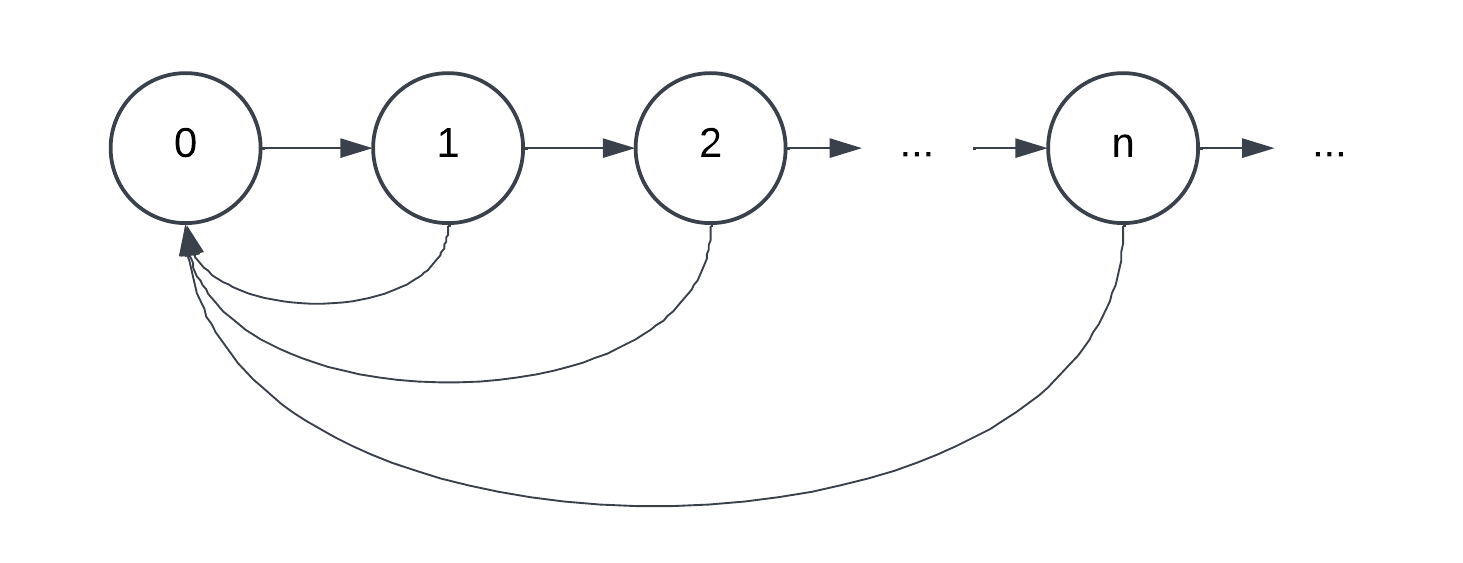
\includegraphics[scale=0.5]{one_part_c_markov_graph.png}
	\caption{
		A graphical representation of the Markov Chain in problem 1 part (c).
	}\label{fig:f3}
\end{figure} \\

\noindent
The one step transition matrix can be written as
\begin{align*}
P =
\begin{bmatrix}
1/6 & 5/6 & 0 & 0 & \dots \\
1/6 & 0 & 5/6 & 0 & \dots \\
1/6 & 0 & 0 & 5/6 & \ddots\\
\vdots & \vdots & \ddots & \ddots & \ddots\\
\end{bmatrix}.
\end{align*}
Once again, observe we have rows that sum to 1 and the probability of moving from one state to another only depends on which state we are currently in. \\
\qed \\


\item At time $n$, $X_n$ is the time until the next six is rolled. \\

\noindent
\textit{Solution:} \\
Suppose $X_1 = k$ meaning we are going to role a 6 in $k$ roles.
Then we know that $X_2 = k - 1, ..., X_k = 1$.
Thus the $k + 1$ role is a 6 and we no longer have definitive information about time until the next 6 will be rolled.
Let's consider $X_{k + 1} = \ell$, $\ell \in \mathbb N$. Then there are going to be $\ell - 1$ non 6 roles followed by a single role of 6.
The probability of $\ell - 1$ non 6 roles is $\big(\frac 5 6 \big)^{\ell - 1}$ then we would multiply by an additional $1/6$.
We can represent this uncertainty for the state of $X_{k+1}$ as 
$$P(X_{k + 1} = \ell) = \bigg(\frac 5 6 \bigg)^{\ell - 1}\frac 1 6.$$
Notice, this is just a geometric distribution.
Therefore, the one step transition matrix can be written as
\begin{align*}
P =
\begin{bmatrix}
1/6 & (5/6)1/6 & (5/6)^2 1/6 & (5/6)^3 1/6 & \dots \\
1 & 0 & 0 & 0 & \dots \\
0 & 1 & 0 & 0 & \ddots\\
0 & 0 & 1 & 0 & \ddots\\
\vdots & \vdots & \ddots & \ddots & \ddots\\
\end{bmatrix}.
\end{align*}
Since the first row of the matrix is just a geometric distribution it sums to 1 and the others sum to 1 trivially.
Additionally, the probability of moving from one state to another is fully determined by the current state, this is indeed a Markov Chain.
\qed \\

\end{enumerate}
\newpage


\noindent {\bf 2.} Exercise 4.2. \\
Let $Y_n = X_{2n}$. Compute the transition matrix for $Y$ when

\begin{enumerate}[(a)]
\item $X$ is a simple random walk (i.e., $X$ increases by one with probability $p$ and decreases by $1$ with probability $q$. \\

\noindent
\textit{Solution:} \\
Let's define the one step transition matrix for the random variable $X$ which is a random walk increasing by 1 or decreasing by 1 with probability $p$ and $q$ respectively.
The entries of the one step transition matrix for $X_n$ are given by
$$
p(i, j) = P(X_{n + 1} = j | X_n = i) = \begin{cases}
p, & j = i + 1\\
q, & j = i - 1 \\
0, & {\rm else}
\end{cases}
$$
Looking at the graph in Figure \ref{fig:f4}, we represent the Markov chain for $X_n$ where moving to the right with probability $p$ and to the left with probability $q$.
\begin{figure}[h]
	\centering
	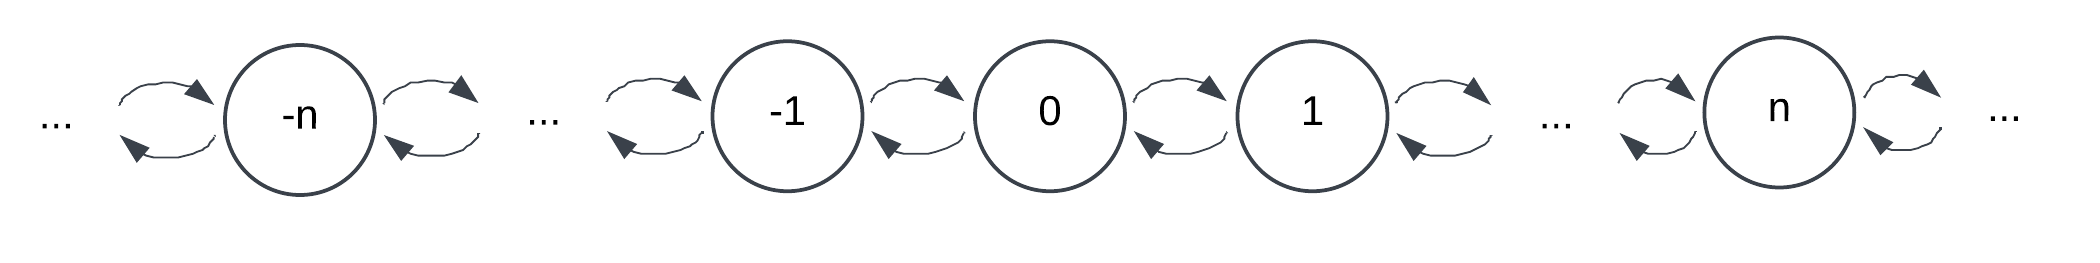
\includegraphics[scale=0.5]{two_part_a_markov_graph.png}
	\caption{
		A graphical representation of the Markov Chain in problem 2 part (a).
	}\label{fig:f4}
\end{figure}
Now we want to represent the one step transition matrix for $Y_n$.
\begin{align*}
p(i, j) = P(Y_{n + 1} = j | Y_n = i) 
= P(X_{2n + 2} = j | X_2n = i) = \begin{cases}
p^2, & j = i + 2\\
q^2, & j = i - 2 \\
2pq, & j = i \\
0, & {\rm else}.
\end{cases}
\end{align*}
This is the representation of the entries of the one state transition matrix for $Y_n = X_{2n}$. \\
\qed \\


\item $X$ is a branching process where $G$ is the generating function of the number of offspring from each individual. \\

\noindent
\textit{Solution:} \\ 
Let's begin by looking at what $p(i, j)$ looks like in the transition matrix for the branching process that $X$ represents.
Without loss of generality and for convenience, we will assume we are beginning with the term $X_{2n} = i$ and asking about the values $X_{2n + 1}$ will take on.
We have
$$
p(i,j) = P(X_{2n + 1} = j | X_{2n} = i).
$$
Recall that in our branching process we define $X_{n + 1}$ as follows
$$
X_{2n+1} = \xi_1 + ... + \xi_{X_{2n}} = \sum_{\ell = 1}^{X_{2n}} \xi_\ell =  \sum_{\ell = 1}^i \xi_\ell.
$$
Furthermore, looking at the generating function we have
$$
G_{X_{2n + 1}}(s) = G_{\sum_{\ell = 0}^i \xi_\ell}(s) = \big(G_\xi(s)\big)^i.
$$
Suppose, $X_{2n+1} = k$.
Then
$$
X_{2n+2} = \xi_1 + \dots + \xi_{X_{2n + 1}} = \sum_{m = 1}^{X_{2n + 1}} \xi_m = \sum_{m = 1}^k \xi_m
$$
Finally, let's look at the generating function of $Y$,
$$
G_{Y_{n + 1}}(s) = G_{k}(G(s)) = \Big( G\big(G(s)\big) \Big)^i.
$$
Using this generating function we can determine the distribution which describes the entries of the one step transition matrix for $Y$ using the formula for distribution from generating function
$$
p(i,j) = \frac {\D^j}{\D s^j} \left[ \frac {\Big( G\big(G(0)\big) \Big)^i}{j!} \right]
$$
\qed \\

\end{enumerate}
\newpage


\noindent {\bf 3.} Exercise 4.3. \\
Let $X$ be a Markov chain with state space $S$ and absorbing state $k$ (i.e., $p(k, j) = 0$ for all $j \in S$).
Suppose $j \rightarrow k$ for all $j \in S$.
Show that all states other than $k$ are transient. \\

\noindent
\textit{Solution:} \\
Assume $X$ is a Markov chain with state space $S$.
This means there exists a one step transition matrix representing the Markov chain transition probabilities.
Additionally, by definition the rows of these matrices should add up to one.
Intuitively this translates to summing up the probability of going to each state you can access in one move from the current state should produce 1. Additionally assume that there exists a state $k \in S$ which is an absorbing state, meaning
$$p(k, j) = 0 \quad \text{ for all } j \in S.$$
Finally assume that every state $j \in S$ communicates with $k$ that is written as $j \rightarrow k$ and means
$$
p_n(j,k) = P(X_n = k | X_0 = j) > 0 \quad \text{ for some } n \geq 1
$$
Figure \ref{fig:f5} may help visualize this a little.
\begin{figure}[h]
	\centering
	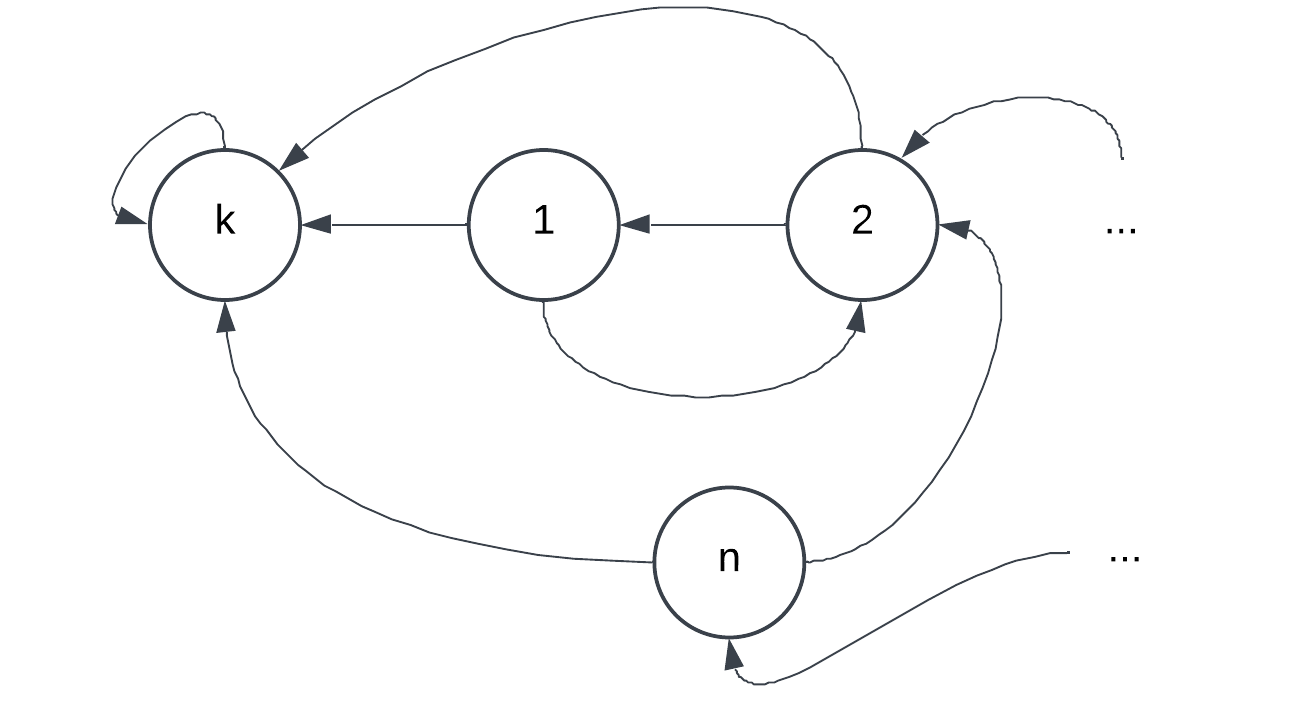
\includegraphics[scale=0.5]{three_markov_graph.png}
	\caption{
		A graphical representation of the Markov Chain in problem 3 which has an absorbing state $k$.
	}\label{fig:f5}
\end{figure}
Assume by way of contradiction that there exists a persistent state $\ell \in S$.
Then $P(X_n = \ell | X_0 = \ell) = 1$ for some $n > 0$.
If this is were true, then we would need $P(X_n = k | X_0 = \ell) = 0$ in order to avoid entering the absorbing state and never being able to leave.
However, this contradicts our assumption that $j \rightarrow k$ for all $j \in S$ which originally indicated
$$
P(X_n = k | X_0 = j) > 0
$$
not equal to 0 as the contradictory assumption led us to believe.
Therefore, $\ell$ must not be a persistent state, which means all states $j \in S$ other than $k$ are transient. \\
\qed \\

\newpage


\noindent {\bf 4.}  Exercise 4.4. \\
Suppose two distinct states $i, j$ satisfy
$$
P(\tau_j < \tau_i | X_0 = i) = P(\tau_i < \tau_j | X_0 = j)
$$
where $\tau_j := {\rm inf}\{n \geq 1: X_n = j\}$.
Show that, if $X_0 = i$, the expected number of visits to $j$ prior to re-visiting $i$ is one. \\

\noindent
\textit{Solution:} \\
Let's first analyze the given information.
In english the first passage time, written as $\tau_j := {\rm inf}\{n \geq 1: X_n = j\}$, is the smallest $n$ such that we arrive at state $j$.
Therefore the information we are given states, if we start in state $i$ the probability that you arrive at state $j$ before arriving at state $i$ again is equal to the probability of arriving at state $i$ before state $j$ given that we start in state $j$ this time.
Apologies for how confusing that may come across in english but It helped me think through the problem being asked.
Figure \ref{fig:f6} may help visualize this a little.
\begin{figure}[h]
	\centering
	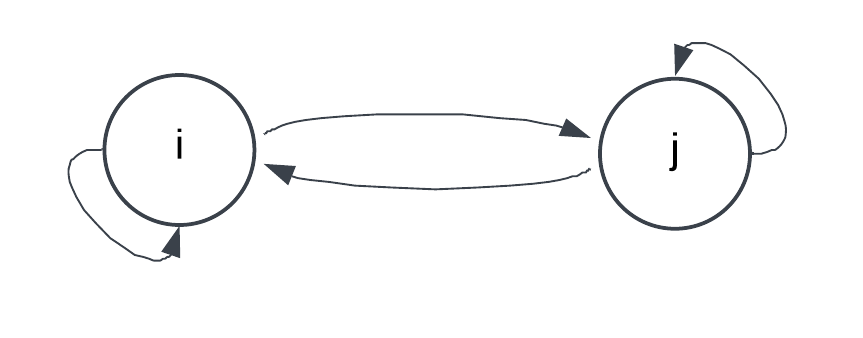
\includegraphics[scale=0.85]{four_markov_graph.png}
	\caption{
		A graphical representation of the Markov Chain in problem 4. Note the directed edges don't necassarily represent immediate paths but rather could include any number of visits to any number of other states in $S$ along the way. For simplicity, we only look at the nodes of interest and supres other possible states from the Markov chain graph visualization.
	}\label{fig:f6}
\end{figure}
Let us define the random variable $Y$ to be equal to the number of times we visit $j$ before re-visiting $i$.
We want to show $E(Y) = 1$.
Notice, the expected value of $Y$ is (skipping change of variables and relying on the fact that we have a discrete but countable random outcome space)
$$
E(Y) = \sum_{y=0}^\infty yP(Y = y) = 0 \cdot P(Y = 0) + \sum_{y=1}^\infty yP(Y = y) = \sum_{y=1}^\infty yP(Y = y).
$$
In order to look more closely at what $P(Y = y)$ will look like we need to define a few more things.
Let $p$ be the probability of starting at $i$ and visiting $j$ before revisiting $i$. And thus $1-p$ be the probability of revisiting $i$ before visiting $j$.
Due to our assumptions about the relationships of the first passage times and starting states, this is the same probabilities changing the role of $j$ and $i$ in the previous statement.
We can update our visual with these probabilities in Figure \ref{fig:f7}.
\begin{figure}[h]
	\centering
	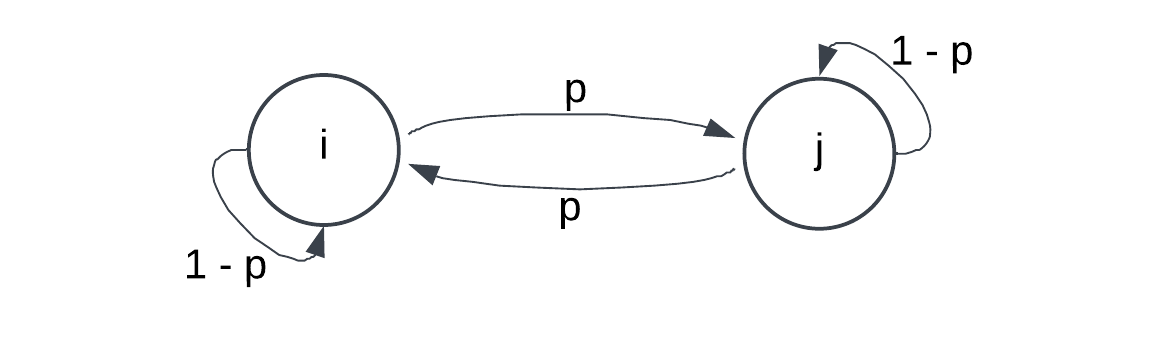
\includegraphics[scale=0.85]{four_with_prob_markov_graph.png}
	\caption{
		A graphical representation of the Markov Chain in problem 4, now with probabilities added.
	}\label{fig:f7}
\end{figure}
Now we can denote the following
\begin{align*}
P(Y = 1) &= p^2 \\
P(Y = 2) &= p^2(1 - p) \\
P(Y = 3) &= p^2(1 - p)^2 \\
& \vdots \\
P(Y = y) &= p^2(1 - p)^{y - 1}
\end{align*}
This relationship comes from the fact that to visit $j$ once and come back to $i$ you have a chance $p$ of going each way hence $p^2$.
Additionally, revisiting $j$ before coming back to $i$ has a probability of $1 - p$ so each time it would do that get's us another power of $1 - p$. combining this with the expectation from earlier we have
\begin{align*}
E(Y) &= \sum_{y=1}^\infty yP(Y = y) \\
	&= \sum_{y=1}^\infty yp^2 (1 - p)^{y- 1} \\
	&= p^2 \sum_{y = 1}^\infty y(1 - p)^{y - 1} \\
	&= p^2 \frac 1 {\big(1 - (1 - p)\big)^2} \\
	&= p^2 \frac 1 {p^2} \\
	&= 1.
\end{align*}
Therefore the expected number of times we visit $j$ before revisiting $i$ given that we start at $i$ is 1. \\
\qed \\

\newpage


\noindent {\bf 5. Stationary distribution of Ehrenfest chain.} (a) Let $X_n$ be the number of balls in the left urn at time $n$ (total number of balls in both urns is $r$). At each time step, one of the $r$ balls is picked at random and moved to the other urn. \\

\noindent
(a) Let $G_n(s)$ be the generating function of $X_n$. Derive a formula for $G_{n+1}$ as a function of $G_n$. \\

\noindent
\textit{Solution:} \\
First, I will establish what the $p(i,j)$'s are for $X_n$ which correspond to the entries of the one state transition matrix.
Define it to be
$$
P(X_{n + 1} = j | X_n = i) = p(i,j) = 
\begin{cases}
(r - i)/r & \text{ if } j = i + 1 \\
i/r & \text{ if } j = i - 1 \\
0 & \text {else}.
\end{cases}
$$
Then from here we can calculate $G_{n+1}(s)$ as follows
\begin{align*}
G_{n+1}(s) &= E\Big( s^{X_{n + 1}} \Big| X_n = i \Big) \\
	&= \sum_{i=0}^r\sum_{j = 0}^r P(X_n = i)P(X_{n + 1} = j | X_n = i) s^{j} \\
	&= \sum_{i=0}^r P(X_n = i) \sum_{j = 0}^r P(X_{n + 1} = j | X_n = i) s^{j} \\
	&= \sum_{i=0}^r P(X_n = i) \left( \frac {r - i} r s^{i +1} + \frac i r s^{i - 1} \right) \\
	&= \frac 1 r \sum_{i=0}^r P(X_n = i) \left( (r - i) s^{i +1} + i s^{i - 1} \right) \\
	&= \frac 1 r \sum_{i=0}^r P(X_n = i) \left( (r - i) s^{i +1} + i s^{i - 1} \right) \\
	&= \frac 1 r \sum_{i=0}^r P(X_n = i) \left( rs^{i +1} - is^{i +1}  + i s^{i - 1} \right) \\
	&= \frac 1 r \sum_{i=0}^r P(X_n = i) rs^{i +1} - \frac 1 r \sum_{i=0}^r P(X_n = i) is^{i +1}  + \frac 1 r \sum_{i=0}^r P(X_n = i) i s^{i - 1} \\
	&= s\sum_{i=0}^r P(X_n = i) s^i - \frac {s^2} r \sum_{i=0}^r P(X_n = i) is^{i - 1}  + \frac 1 r \sum_{i=0}^r P(X_n = i) i s^{i - 1} \\
	&= sG_n(s) - \frac {s^2} r G_n^{\prime}(s)  + \frac 1 r G_n^{\prime}(s).
\end{align*}
\qed \\
\newpage

\noindent
(b) Let $G(s)= \lim_{n \to \infty}  G_n(s)$. Use the relation in part a) to derive an equation for $G$. Solve it and find $G$. \\

\noindent
\textit{Solution:} \\
Taking the limit of $G_{n + 1}(s)$ as $n$ goes to infinity we have
\begin{align*}
G(s) &= sG(s) + \frac 1 r (1 - s^2)G^\prime(s) \\
G(s) - sG(s) &= \frac 1 r (1 - s^2)G^\prime(s) \\
\left(G(s) - sG(s)\right)\frac r {(1 - s^2)}  &= G^\prime(s) \\
G(s) \cancel{(1 - s)}\frac r {\cancel{(1 - s)}(1 + s)}  &= G^\prime(s) \\
G(s) \frac r {1 + s}  &= G^\prime(s).
\end{align*} 
To solve this differential equation we can do the following
\begin{align*}
\frac {G^\prime(s)} {G(s)} &= \frac r {1 + s} \\
\int \frac {G^\prime(s)} {G(s)} \D s&= \int \frac r {1 + s} \D s \\
\log G(s) &= \int \frac r {1 + s} \D s \\
\log G(s) &= r \log(1 + s) + C \\
\log G(s) &= \log\big((1 + s)^r\big) + C \\
G(s) &= \E^{\log\big((1 + s)^r\big) + C} \\
G(s) &= (1 + s)^r\E^C \\
G(s) &= (1 + s)^rC_1.
\end{align*}
The initial condition we can use to help here is that $G(1) = 1$
Therefore
\begin{align*}
G(0) &= (1 + 1)^rC_1 \\
1 &= 2^r C_1 \\
\frac 1 {2^r} &= C_1
\end{align*}
Hence
$$
G(s) = (1 + s)^r \frac 1 {2^r}.
$$
\qed \\

\noindent
(c) Find the stationary distribution $\pi$ of Ehrenfest chain. What is the connection between $G$ and $\pi$? \\

\noindent
\textit{Solution:} \\
\textbf{TODO: Didn't get time to come back to this} \\

\newpage




\end{document}  
